\chapter{Machine learning based approach}


%====================================================================================================
\section{Concepts in machine learning}
Aim of this section is to define what exactly is understood by a term machine learning as well
as to introduce basic concepts that are common for all machine learning applications

%----------------------------------------------------------------------------------------------------
\subsection{Differences between knowledge and data based models}
While creating a model of physical processes one of two approaches may be used.
First, is the knowledge-driven model that as the name implies relays on knowledge of underlying
laws of physics that govern the process.
The main advantage of this approach is its high explainability and reliability as every parameter
of the model corresponds with some specific physical property.
However this model has a very significant downside, it requires detailed knowledge of physical
phenomena. This means that for complex processes it might be very difficult or even
impossible, at a~given moment, to create a model. Another drawback is that the complexity of
the process grows the computational cost of its model.
If those problem makes creating usable knowledge-based model impossible or economically
non efficient a data-driven approach may be used.
It model used is chosen arbitrarily with little or no relation to underlying physics,
then model parameters are adjusted until it will fit experimental data to the best of its
capability.
The main advantage of a data-driven approach is the lack of required knowledge on process 
inner workings, which allow prediction of events which exact mechanics have not 
yet been discovered.
Another element characteristic in the data-driven approach, that can be either advantageous or
disadvantageous, is the lack of direct correlation between the complexity 
of the process and computational cost of the model.
This is a very welcome trait for complex processes like orbital atomic clock ensembles.
The main disadvantage in comparison with the knowledge-driven approach is its lower reliability and
explainability. This is the main reason why the data-driven approach is usually avoided in
critical implementations. Another significant downside is a requirement of a large amount of
experimental data for model adjustment which means that in many cases this approach simply
cannot be used.
The last thing that must be said about the data-driven approach is that it still requires some
amount of knowledge to work efficiently as the selection of models that will be adjusted to
data requires some assumption. For example, the use of linear regression assumes that the model
is linear.

%----------------------------------------------------------------------------------------------------
\subsection{What is a machine learning algorithm}
Term machine learning describes subset of algorithms that adjusts parameter of other algorithms 
according to data. To provide more formal definition an algorithm can be described as a 
transformation function $\phi_{a}$ such that:
\begin{equation}
	\label{equ:algorithm_general}
	\mathcal{Y}_{a} = \phi_{a}(\mathcal{X},\Theta_{a}),
\end{equation}
where $\mathcal{Y}_{a}$ is set of algorithm responses, $\mathcal{X}$ is set of inputs 
and $\Theta_{a}$ is algorithm parameter set.
Input space $\mathcal{U}_{x}$ and response space $\mathcal{U}_{y}$ can be simply a numerical
space, in which case algorithm is called numerical algorithm, but can also represent more 
abstract concepts. For example in case of database software input space will consist of 
queries while response space will contain information stored in database as well as error 
status in case query was written incorrectly.
Machine learning algorithm, denoted as $\phi_{m}$ can also be described in that general form
however what is special in this case is that input space $\mathcal{U}_{m}$ consists of either :
\begin{equation}
	\label{equ:supervised_input}
	\mathcal{X}_{m} = \{\phi_{a}, \mathcal{X}_{a}, \mathcal{Y}_{a}, \Theta_{a} \},
\end{equation}
in case of supervised learning or just :
\begin{equation}
	\label{equ:supervised_input}
	\mathcal{X}_{m} = \{\phi_{a}, \mathcal{X}_{a}, \Theta_{a} \},
\end{equation}
in case of unsupervised learning.
In both cases response of machine learning algorithm is described as a:
\begin{equation}
	\label{equ:ml_response}
	\mathcal{Y}_{m} = \{\hat{\Theta}_{a}, E_{a}\},
\end{equation}
where $\hat{\Theta}_{a}$ is adjusted set of parameters and $E_{a}$ is value prediction 
error for this new set of parameters.
Aim of machine learning algorithm is to adjust parameters $\Theta_{a}$ of given algorithm 
$\phi_{a}$ in such a way to minimize error $E_{a}$ for given data. In case of supervised learning
a correct response $\mathcal{Y}_{a}$ for inputs is known where in case of unsupervised learning
only input set $\mathcal{X}_{a}$ is known. In order to avoid confusion parameters of machine 
learning algorithm $\Theta_{m}$ will be referred to as a \textit{metaparameters}. 
Exact set of meteaparameters vary between specific algorithms, however there is one 
crucial metaparameter that will appear in every machine learning algorithm.
That metaparameter is error function as it is required for error value calculation and as 
minimization of that value is goal of machine learning it is mandatory to be able to calculate it.

%----------------------------------------------------------------------------------------------------
\subsection{Error function}
As an error function is used for calculation of value that will be minimized by a machine 
learning algorithm correct choice of that function is crucial decision when designing such
algorithm.
Due to scope of this work attention will be given only to error function used in supervised 
learning of numerical algorithms.
Error for single pair of predicted value $\hat{y}$ and actual value $y$ can be described as
distance between them in response space $\mathcal{U}_{y}$:
\begin{equation}
	\label{equ:dist_general}
	E = f_{DIST}(\hat{y},y),
\end{equation}
where $f_{DIST}$ is distance function, alternatively called metric.
Distance function is a function that gives a distance between each pair of point elements of a set.
If a set have a distance function defined it is called a metric space. 
In order to be classified as a metric function $f_{DIST}$ over a Cartesian square of a universe 
$\mathcal{U}$ it must display following properties:
\begin{enumerate}
	\item $f_{DIST} : \mathcal{U} \times \mathcal{U} \to \mathbb{R}^{+}$
	\item identity of indiscernibles : $f_{DIST}(x_{0}, x_{1})=0 \leftrightarrow x_{0} = x_{1}$,
	\item symmetry : $f_{DIST}(x_{0},x_{1})=f_{DIST}(x_{1},x_{0})$,
	\item triangle inequality : $f_{DIST}(x_{0},x_{1}) \leq f_{DIST}(x_{0},x_{2}) +
		f_{DIST}(x_{1},x_{2})$. 
\end{enumerate}

There are many types of metrics however within scope of this work attention will be given only to
distance functions related to $\ell$ norms.
As such error function for single prediction will be described as: 
\begin{equation}
	\label{equ:dist_norm}
	E = \Vert (\hat{y}-y) \Vert_{k},
\end{equation}
where notation $\Vert \bullet \Vert_{k}$ describes $k$ norm of given value.
Norm is a function from a real or complex vector space to the non negative real number space
that describes distance of a point from the origin.
Origin is the point for which values of all dimension are equal to zero, in case of calculating
$\ell$ norm for difference between two points subtrahend is treated as a origin point.
General equation describing a $\ell_{k}$ norm in $n$ dimensional space is:
\begin{equation}
	\label{equ:ell_norm}
	\Vert x \Vert_{k} = (\vert x_{0} \vert^{k} + \vert x_{1} \vert^{k} + \cdots +
	\vert x_{n} \vert^{k})^{1/k},
\end{equation}
where $\vert x \vert$ is an absolute value of $x$.
\begin{figure}[htb] 
	\label{fig:l_norms}
	\centering
	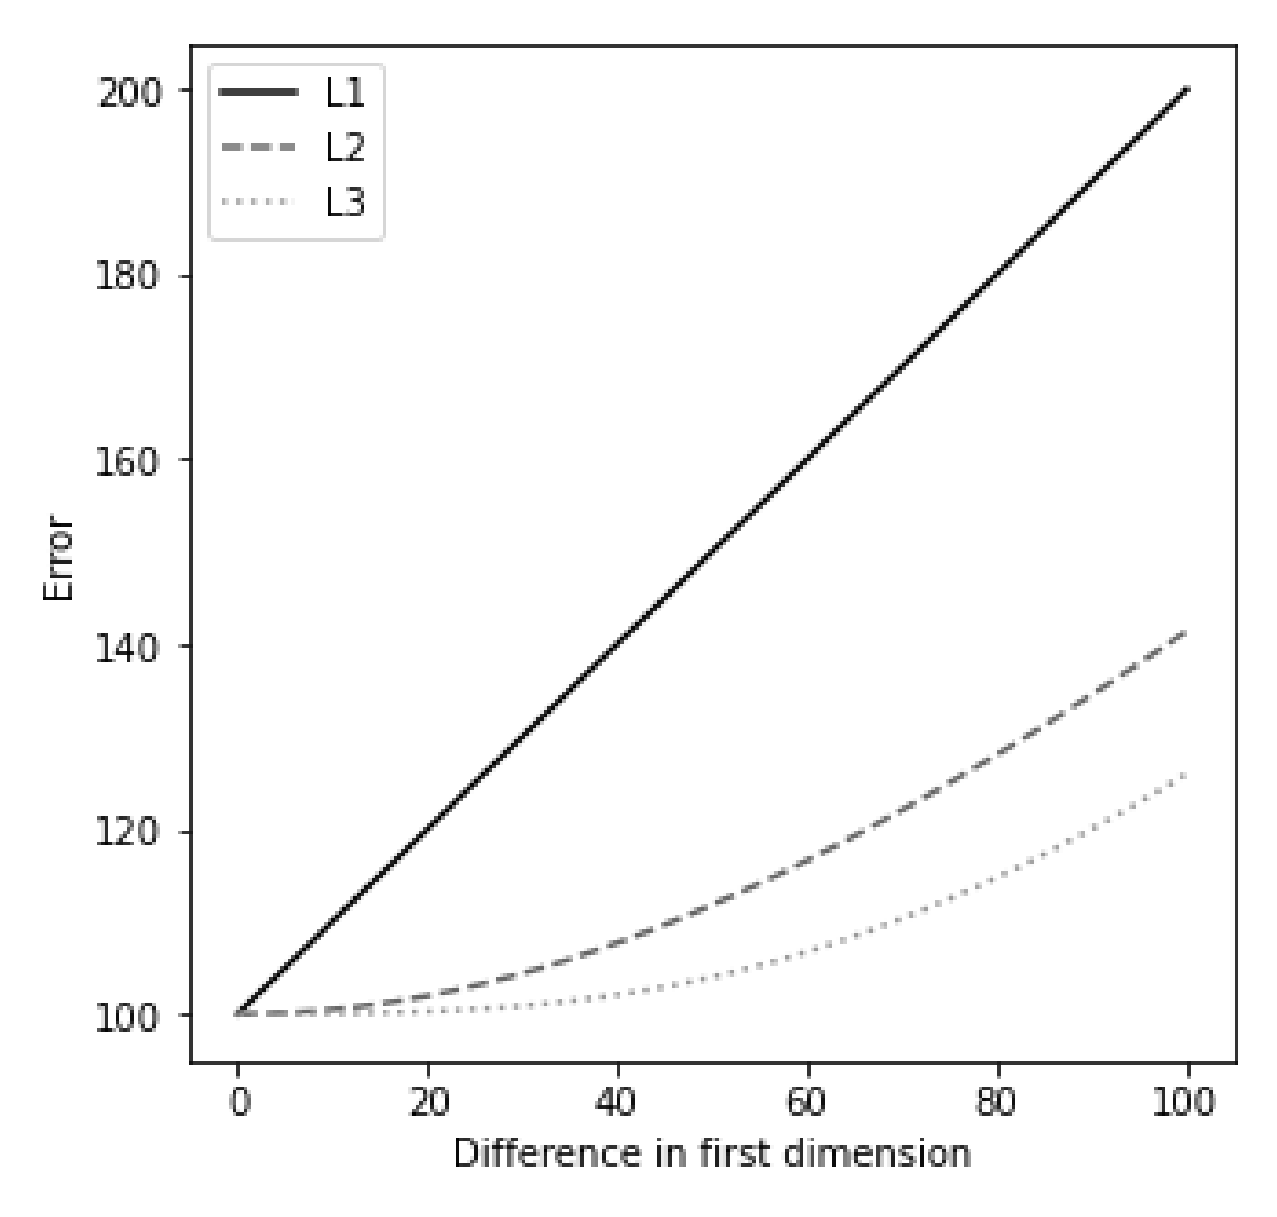
\includegraphics[width=0.5\textwidth]{figures/l_norms}
	\caption{Relation between error and difference in first dimension values with second 
	dimension difference at constant 100}
\end{figure}
\textbf{TODO: DESCRIBE WHY USE GIVEN NORMS IN MORE DETAIL}
Norms usually used in error calculation are $\ell_{1}$ and $\ell_{2}$, due to their frequent use
not only in this field they are given specific names.
Norm $\ell_{2}$ is called Euclidean norm and is equivalent to intuitive understanding of distance
while norm $\ell_{1}$ is called Manhattan distance and is related to distance between points on 
grid.
Euclidean distance is used for calculation of Root Mean Squared Error (RMSE). If we define 
knowledge base $K$ as a set of pairs $(x,y)$ where $x$ is input and $y$ an expected output
while prediction is realised by hypothesis $\hat{y} = h(x,\phi)$ error can be described as:
\begin{equation}
	\label{equ:mse}
	f_{RMSE}(K,h) = \sqrt{\frac{1}{\vert K \vert} \sum_{(x,y) \in K}(h(x,\phi)-y)^2},
\end{equation}
where $\vert K \vert$ is cardinality of knowledge base.
Manhattan distance is in turn used to calculate Mean Average Error (MAE):
\begin{equation}
	\label{equ:mae}
	f_{MAE}(K,h) = \frac{1}{\vert K \vert} \sum_{(x,y) \in K}\vert (h(x,\phi)-y)\vert.
\end{equation}
Those two error values will be used in this work.


%----------------------------------------------------------------------------------------------------
\subsection{Deep learning}
At time when experiments described in this dissertation were conducted a new approach to 
machine learning called Deep Learning (DL) became highly popular.
Due to that popularity term deep learning is often overused and misrepresented marketing 
purposes. In this section an attempt will be made to explain what exactly constitutes as a
deep learning and describe what sort of challenges.
Term deep learning can be applied only to a subset of machine learning algorithms that have
layer based architecture, usually a neural networks.
In such implementation whole data processing algorithm can be described as a transformation:
\begin{equation}
	\label{equ:spaces1}
	\phi = \mathcal{U}_{OBS} \Rightarrow \mathcal{U}_{RES},
\end{equation}
where $\mathcal{U}_{OBS}$ is called observation space and $\mathcal{U}_{RES}$ is response space.
In case of simple single layer system observation space is directly transformed into a 
response space, however in case of multi layer model there are intermediate encoding spaces.
In such case representation spaces are numbered by index of layer which outputs them. 
So in case of $n$ layer system it would be $\{\mathcal{U}_{0}, \mathcal{U}_{1},
\cdots, \mathcal{U}_{n}\}$ where indexes $0$ and $n$ are special as 
$\mathcal{U}_{0}=\mathcal{U}_{OBS}$ and $\mathcal{U}_{n}=\mathcal{U}_{RES}$.
In that case a function transforming observation into a reaction can be described as a 
convolution of multiple encoding function.
\begin{equation}
	\label{equ:spaces_transform}
	\phi = \phi_{1} \otimes \phi_{2} \otimes \cdots \otimes \phi_{n}.
\end{equation}
Transformation $\phi_{n}$ is called output layer, while other transformation are referred to
as a hidden layers as their result is not visible during normal operation of algorithm.
Until recently almost all architectures used a single hidden layer and architectures with more
than 3 hidden layers were almost unheard of.
This is due to three issue that show up in systems with higher amount of layer: signal vanishing,
signal explosion and rise in computation due to high parameter count.


%====================================================================================================
\section{Regression approximation}

%----------------------------------------------------------------------------------------------------
\subsection{Linear regression}
\label{sec:linear_regression}
Linear predictor function is a linear combination of a set of coefficients and explanatory 
variables (independent variables), whose value is used to predict the outcome of a
dependent variable. Linear predictor is described as:
\begin{equation}
	\label{equ:linear_predictior}
	\hat{y} = \Theta_{0} + \Theta_{1}x_{1} + \cdots + \Theta_{n}x_{n},
\end{equation}
where $\hat{y}$ is predicted value,$n$ is feature count, $x_{i}$ is value of i-th feature
and $\Theta_{j}$ is j-th parameter.
Parameter $\Theta_{0}$ is special as it is not corresponding to any feature, that parameter
is called a \textit{bias term} or just \textit{bias}.
Predictor will return value of bias if all inputs are set to zero.
Function that allows prediction is called hypotesis function and is written as $\hat{y} = h(x)$.
With assumption that input vector for such function is $x=[1, x_{1}, \cdots, x_{n}]$ then 
a hypotesis function of a linear predictor can be defined as:
\begin{equation}
	\label{equ:linear_hyp}
	\hat{y} = h_{\Theta}(x) = \Theta^{T}\cdot x.
\end{equation}
To define how well prediction fit actuall data a error function must be selected and then one
of to approaches for minimizing it must be applied. Gradient based approach will be described 
is section \ref{sec:gradient} here a analytical approach based on a normal equation will be shown.
To derieve normal equation a MSE will be used as a error function, if other function would be 
selected a different normal equation would be a result.
In matrix notation hypothesis function can be described as :
\begin{equation}
	\label{equ:linear_hyp_matirx}
	\hat{Y} = h_{\Theta}(X) = \Theta^{T}\cdot X,
\end{equation}
where $X$ is input matrix such that each row represent single observation and each column 
single feature:
\begin{equation}
	\label{equ:input_matrix}
	X_{m\times m}=\left( \begin{array}{c c c c c}
		1& x^{(1)}_{1}& x^{(1)}_{2}& \cdots& x^{(1)}_{n}\\
		1& x^{(2)}_{1}& x^{(2)}_{2}& \cdots& x^{(2)}_{n}\\
		1& x^{(3)}_{2}& x^{(3)}_{2}& \cdots& x^{(3)}_{n}\\
		\vdots&\vdots&\vdots&\ddots&\vdots\\
		1& x^{(m)}_{2}& x^{(m)}_{3}& \cdots& x^{(m)}_{n}\\
	\end{array}\right),
\end{equation}
where $x^{(i)}_{j}$ denotes value of $j$ feature of $i$ observation.
Using this definitions the least-squares error function can be represented in matrix form as:
\begin{equation}
	\label{equ:mse_matrix}
	f_{MSE}(X,y) = \frac{1}{2m}(X\Theta - y)^{T}(X\Theta - y), 
\end{equation}
where $y$ is column vector of expected responses.
For puproses of of minimization the constans scaling factor $\frac{1}{2m}$ can be ignored, it is
guaranteed that $m\neq 0$ as there is no meaning of learning for zero observations.
With that following transformations of equation can be made:
\begin{equation}
	\label{equ:mse_transform1}
	f_{MSE}(X) = ((X\Theta)^{T} - y^{T})^{T}(X\Theta - y), 
\end{equation}
\begin{equation}
	\label{equ:mse_transform2}
	f_{MSE}(X) = (X\Theta)^{T}X\Theta-(X\Theta)^{T}y-y^{T}(X\Theta)+y^{T}y.
\end{equation}
This can be even further simplified to:
\begin{equation}
	\label{equ:mse_transform2}
	f_{MSE}(X) = \Theta^{T}X^{T}X\Theta-2(X\Theta)^{T}y+y^{T}y. 
\end{equation}
As $\theta$ is the unknown that is being minimised $f_{MSE}$ have to be derived by $\theta$
and compared to 0.
Result od that deriviation is:
\begin{equation}
	\label{equ:mse_derived}
	\frac{\partial J}{\partial \Theta} = 2X^{T}X\Theta - 2X^{T}y = 0,
\end{equation}
form that an equation it is simple to derieve a normal equation that allows calculation of 
$\Theta$:
\begin{equation}
	\label{equ:mse_derived}
	\Theta = (X^{T}X)^{-1}X^{T}y.	
\end{equation}


Standard linear regression models with standard estimation techniques make a number of 
assumptions about the predictor variables, the response variables and their relationship.
Numerous extensions have been developed that allow each of these assumptions to be relaxed 
(i.e. reduced to a weaker form), and in some cases eliminated entirely. 
Generally these extensions make the estimation procedure more complex and time-consuming,
and may also require more data in order to produce an equally precise model.

Example of a cubic polynomial regression, which is a type of linear regression. 
Although polynomial regression fits a nonlinear model to the data, as 
a statistical estimation problem it is linear, in the sense that the regression 
function E(y | x) is linear in the unknown parameters that are estimated from the data. 
For this reason, polynomial regression is considered to be a special case of 
multiple linear regression.

The following are the major assumptions made by standard linear regression models with 
standard estimation techniques (e.g. ordinary least squares):

\begin{enumerate}
    \item Weak exogeneity. This essentially means that the predictor variables x 
		can be treated as fixed values, rather than random variables. 
		This means, for example, that the predictor variables are assumed to be error-free—that 
		is, not contaminated with measurement errors. 
		Although this assumption is not realistic in many settings, dropping it leads to
		significantly more difficult errors-in-variables models.
    \item Linearity. This means that the mean of the response variable is a linear combination 
		of the parameters (regression coefficients) and the predictor variables.
		Note that this assumption is much less restrictive than it may at first seem. 
		Because the predictor variables are treated as fixed values (see above), linearity is
		really only a restriction on the parameters. 
		The predictor variables themselves can be arbitrarily transformed, and in fact multiple
		copies of the same underlying predictor variable can be added, each one transformed 
		differently. This technique is used, for example, in polynomial regression, 
		which uses linear regression to fit the response variable as an arbitrary polynomial 
		function (up to a given rank) of a predictor variable.
		With this much flexibility, models such as polynomial regression often have
		"too much power", in that they tend to overfit the data. As a result,
		some kind of regularization must typically be used to prevent unreasonable solutions
		coming out of the estimation process. 
		Common examples are ridge regression and lasso regression. Bayesian linear regression 
		can also be used, which by its nature is more or 
		less immune to the problem of overfitting.
    \item Constant variance (a.k.a. homoscedasticity). This means that the variance of 
		the errors does not depend on the values of the predictor variables.
		Thus the variability of the responses for given fixed values of the predictors is the
		same regardless of how large or small the responses are. 
		This is often not the case, as a variable whose mean is large will typically have a 
		greater variance than one whose mean is small.
\end{enumerate}
To check for violations of the assumptions of lineaarity, constant variance, and independence
of errors within a linear regression model, the residuals are typically plotted against the 
predicted values (or each of the individual predictors). 
An apparently random scatter of points about the horizontal midline at 0 is ideal, 
but cannot rule out certain kinds of violations such as autocorrelation in the errors or their 
correlation with one or more covariates.
Independence of errors. This assumes that the errors of the response variables are uncorrelated 
with each other.
(Actual statistical independence is a stronger condition than mere lack of correlation and is 
often not needed, although it can be exploited if it is known to hold.) 
Some methods such as generalized least squares are capable of handling correlated errors, 
although they typically require significantly more data unless some sort of regularization is used 
to bias the model towards assuming uncorrelated errors. Bayesian linear regression is a general 
way of handling this issue.
Lack of perfect multicollinearity in the predictors. 
For standard least squares estimation methods, the design matrix X must have full column rank p; 
otherwise perfect multicollinearity exists in the predictor variables, meaning a linear 
relationship exists between two or more predictor variables. 
This can be caused by accidentally duplicating a variable in the data, using a linear 
transformation of a variable along with the original 
(e.g., the same temperature measurements expressed in Fahrenheit and Celcius), or including a 
linear combination of multiple variables in the model, such as their mean. 
It can also happen if there is too little data available compared to the number of 
parameters to be estimated (e.g., fewer data points than regression coefficients). 
Near violations of this assumption, where predictors are highly but not perfectly correlated, 
can reduce the precision of parameter estimates (see Variance inflation factor). 
In the case of perfect multicollinearity, the parameter vector $\beta$ will be non-identifiable—it 
has no unique solution. In such a case, only some of the parameters can be identified 
(i.e., their values can only be estimated within some linear subspace of 
the full parameter space Rp). See partial least squares regression. 
Methods for fitting linear models with multicollinearity have been developed,
some of which require additional assumptions such as "effect sparsity"—that a large 
fraction of the effects are exactly zero.
Note that the more computationally expensive iterated algorithms for parameter estimation, 
such as those used in generalized linear models, do not suffer from this problem.

%----------------------------------------------------------------------------------------------------
\subsection{Polynomial regression}

%----------------------------------------------------------------------------------------------------
\subsection{Support vector machine}


%====================================================================================================
\section{Gradient based optimization}
\label{sec:gradient}

%====================================================================================================
\section{Neural networks}

%----------------------------------------------------------------------------------------------------
\subsection{Artificial representation of biological neuron}
A neuron or nerve cell is an electrically excitable cell that communicates with other
cells via specialized connections called synapses. 
Neurons are typically classified into three categories based on their function:
\begin{enumerate}
	 \item sensory neurons that respond to stimuli and they send signals to the spinal cord or
		 directly to brain, 
	\item motor neurons that receive signals from the brain and spinal cord to control body
		effectors like muscles or glandular output,
	\item interneurons that connect neurons to other neurons within the same region of the brain 
		or spinal cord.
\end{enumerate}
As neuron is first and foremost a cells it consists of a soma (cell body), dendrites, and a 
single axon. The soma is usually compact. The axon and dendrites are filaments that extrude 
from it. Dendrites typically branch profusely and extend a few hundred micrometers from the soma.
The axon leaves the soma at a swelling called the axon hillock, and travels for as far as 1 meter 
in humans or more in other species. It branches but usually maintains a constant diameter.
At the farthest tip of the axon's branches are axon terminals, where the neuron can transmit
a signal across the synapse to another cell.
Neurons may lack dendrites or have no axon. The term neurite is used to describe either a dendrite
or an axon, particularly when the cell is undifferentiated.

Most neurons receive signals via the dendrites and soma and send out signals down the axon.
At the majority of synapses, signals cross from the axon of one neuron to a dendrite of another.
However, synapses can connect an axon to another axon or a dendrite to another dendrite.
\begin{figure}[htb] 
	\label{fig:neurons}
	\centering
	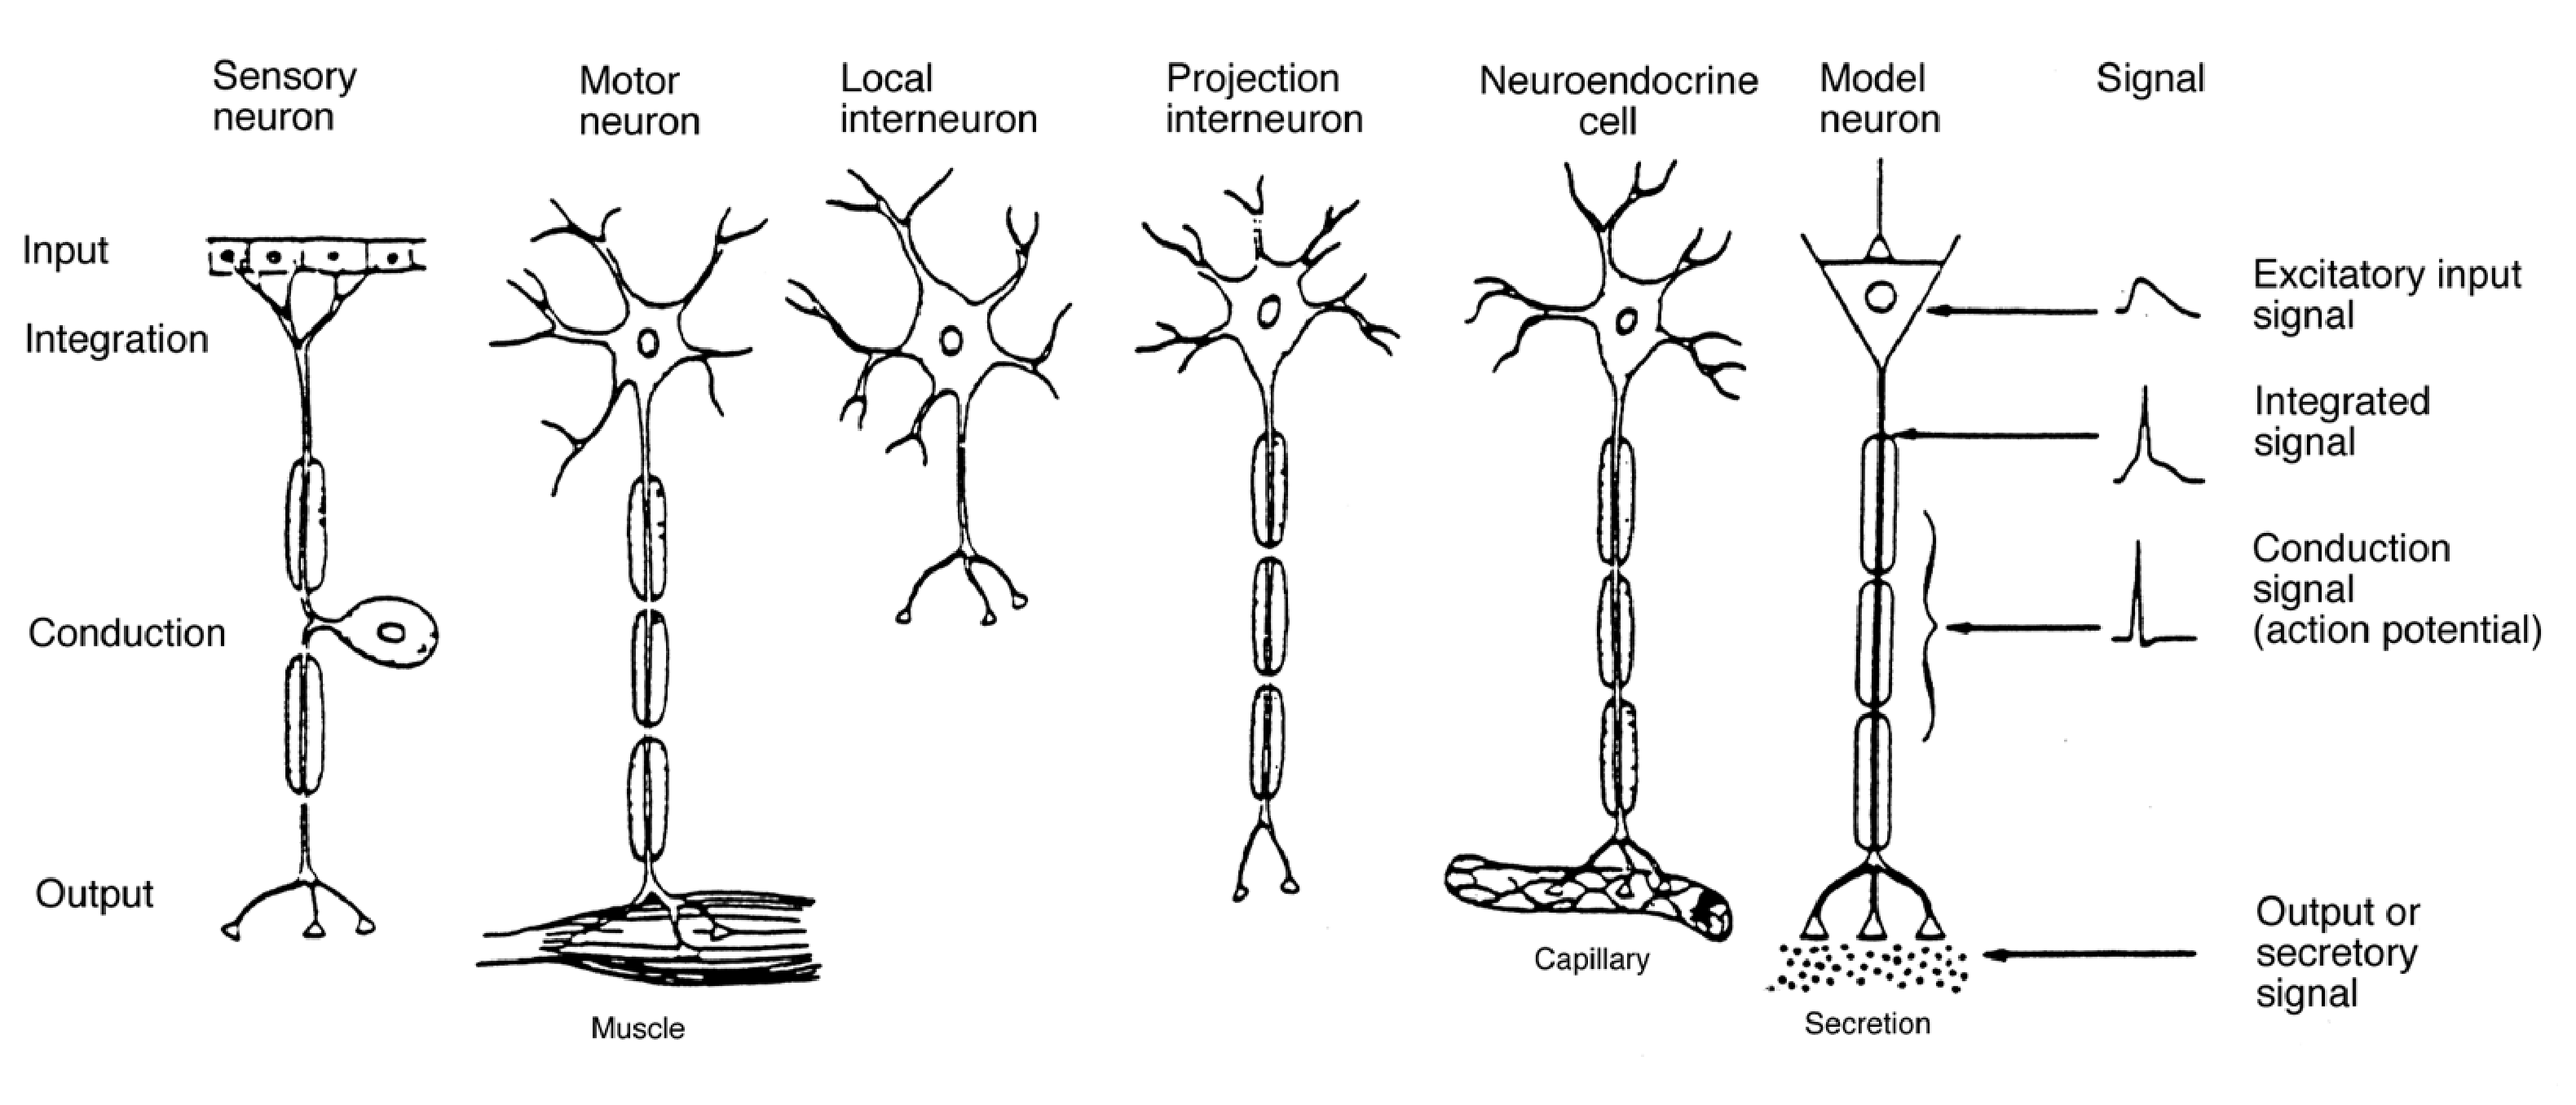
\includegraphics[width=\textwidth]{figures/bio_neurons}
	\caption{Examples of biological neurons}
\end{figure}

The signaling process is partly electrical and partly chemical. Neurons are electrically 
excitable, due to maintenance of voltage gradients across their membranes. 
If the voltage changes by a large enough amount over a short interval, 
the neuron generates an all-or-nothing electrochemical pulse called an action potential. 
This potential travels rapidly along the axon, and activates synaptic connections as it 
reaches them. Synaptic signals may be excitatory or inhibitory, 
increasing or reducing the net voltage that reaches the soma.
\begin{figure}[htb] 
	\label{fig:bio_activation}
	\centering
	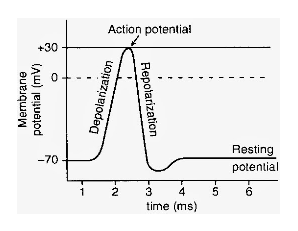
\includegraphics[width=0.6\textwidth]{figures/bio_activation}
	\caption{Examples of biological neurons}
\end{figure}

In 1943 Warren S. McCulloch, a neuroscientist, and Walter Pitts, a logician, 
published "A logical calculus of the ideas immanent in nervous activity" in the 
Bulletin of Mathematical Biophysics 5:115-133. In this paper McCulloch and Pitts tried to
understand how the brain could produce highly complex patterns by using many basic cells
that are connected together. 
McCulloch Pitts neuron is a highly simplified model of neural cell that models only a most
basic behavior of electrical signal transmition.
Neuron is divided into three blocks:
\begin{enumerate}
	\item aggregation where many input signals $\{x_{1}, x_{2}, \cdots, x_{n}\}$ are 
		aggregated into single signal $\hat{u}$,
	\item dampening where signal strength is reduced according to bias term and dampened 
		response $u$ is returned,
	\item activation where signal $u$ is transformed to neuron response space.
\end{enumerate}
Response of neuron modelled like that can be written as:
\begin{equation}
	\label{equ:neuron_response}
	h_{x} = f_{a}(u(\hat{u}(x))),
\end{equation}
however as in most cases weighted sum is realisation of aggregation and dampening is handled by
a simple substation neuron equation is simplified to: 
\begin{equation}
	\label{equ:neuron_response}
	h_{x} = f_{a}(u(x)).
\end{equation}
In case of McCulloch Pitts neuron both aggregation and dampening are realised by a single 
linear function akin to linear predictor:
\begin{equation}
	\label{equ:linear_neuron}
	u(x) = \Theta_{0} + \Theta_{1}x_{1} + \cdots + \Theta_{n}x_{n},
\end{equation}
which as described in chapter \ref{sec:linear_regression} can be written in a matrix notation as
\begin{equation}
	\label{equ:linear_neuron_matrix}
	u(X) = \Theta^{T}\cdot X.
\end{equation}
Almost all modern implementations of artificial neural networks use this aggregation, dampening
model and the only difference between them is in an activation function.
McCulloch Pitts neuron uses step function as an activation:
\[
	\label{equ:step_function}
	 f_{STEP}(u)=
	\begin{cases}
		1,  u > 0, \\
		0,  u \leq 0,
	\end{cases}
	.
\]
With this function neuron can process signals however it still lacks a very important function
of a biological neuron, ability to learn. First learning algorithm developed on base of 
McCulloch Pitts neuron was perceptron algorithm created by \textbf{TODO: BY WHO}.
With $\hat{y}$ defined as a neuron prediction and $y$ as a expected output perceptron learning
algorithm can me described as:
\begin{enumerate}
	\item if $\hat{y}=y$ then do nothing,
	\item if $\hat{y}=1$ and $y=0$ then $\Theta \leftarrow \Theta + x$
	\item if $\hat{y}=0$ and $y=1$ then $\Theta \leftarrow \Theta - x$
\end{enumerate}
Due to its ability to separate space into two subspaces perceptron can be used to model a logical
operators and as such realise logical reasoning.
Let's start with the AND operator.  Looking back at the logic table for the $A\land B$, 
we can see that we only want the neuron to output a 1 when both inputs are activated.
To do this, we want the sum of both inputs to be greater than the threshold, but each input alone
must be lower than the threshold.  Let's use a threshold of 1. 
So, now we need to choose the weights according to the constraints I've just explained - 
how about 0.6 and 0.6?  With these weights, individual activation of either input A or B will 
not exceed the threshold, while the sum of the two will be 1.2, which exceeds the threshold 
and causes the neuron to fire.
I've used a greek letter theta to denote the threshold, which is quite common practice. 
A and B are the two inputs.  You can think of them as input neurons, like photoreceptors, 
taste buds, olfactory receptors, etc.  They will each be set to 1 or 0 depending upon the truth of
their proposition.  The red neuron is our decision neuron. 
If the sum of the synapse-weighted inputs is greater than the threshold, 
this will output a 1, otherwise it will output a 0.  
So, to test it by hand, we can try setting A and B to the different values in the 
truth table and seeing if the decision neuron's output matches the $A\land B$ column:
\begin{itemize}
	\item  $A=0 \land B=0  \to   \hat{y} = 0*1  +  0*1 - 1  = -1 \to$,
	\item $A=0 \land B=1  \to  \hat(y) = 0*1  +  1*1  = 0.6$,
	\item $A=1 \land B=0  \to  \hat(y) = 1*1  +  0*1  = 0.6$,
	\item $A=1 \land B=1  \to  \hat(y) = 1*1  +  1*1  = 1.2$.
\end{itemize}

We have designed a neuron which implements a logical AND gate.  

This is easy to implement in Excel.  In fact, it's exactly the same as the neuron we 
created in What does a neuron do.  

Next up is the OR gate.  Look back at the logic table.  In this case, we want the output to 
be 1 when either or both of the inputs, A and B, are active, but 0 when both of the inputs are 0.  
This is simple enough.  If we make each synapse greater than the threshold, 
then it'll fire whenever there is any activity in either or both of A and B.
This is shown on the right.  Synaptic values of 1.1 are sufficient to surpass 
the threshold of 1 whenever their respective input is active.  
	

%----------------------------------------------------------------------------------------------------
\subsection{Feed forward neural networks}

\begin{figure}[htb] 
	\label{fig:xor_gates}
	\centering
	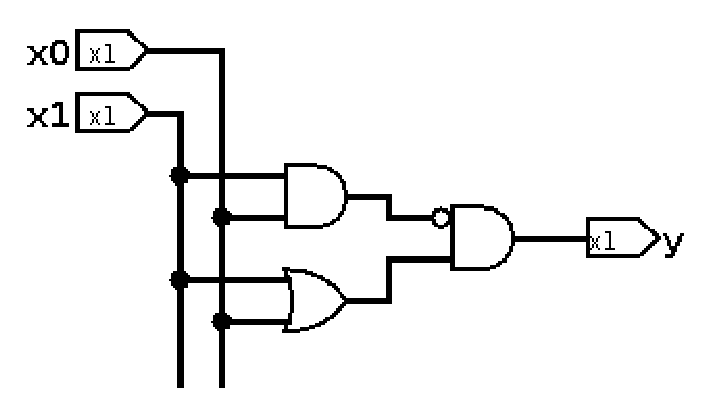
\includegraphics[width=0.6\textwidth]{figures/xor_gates}
	\caption{Implementation of XOR gate with AND, OR and NOT gates}
\end{figure}

\begin{figure}[htb] 
	\label{fig:neuro_xor}
	\centering
	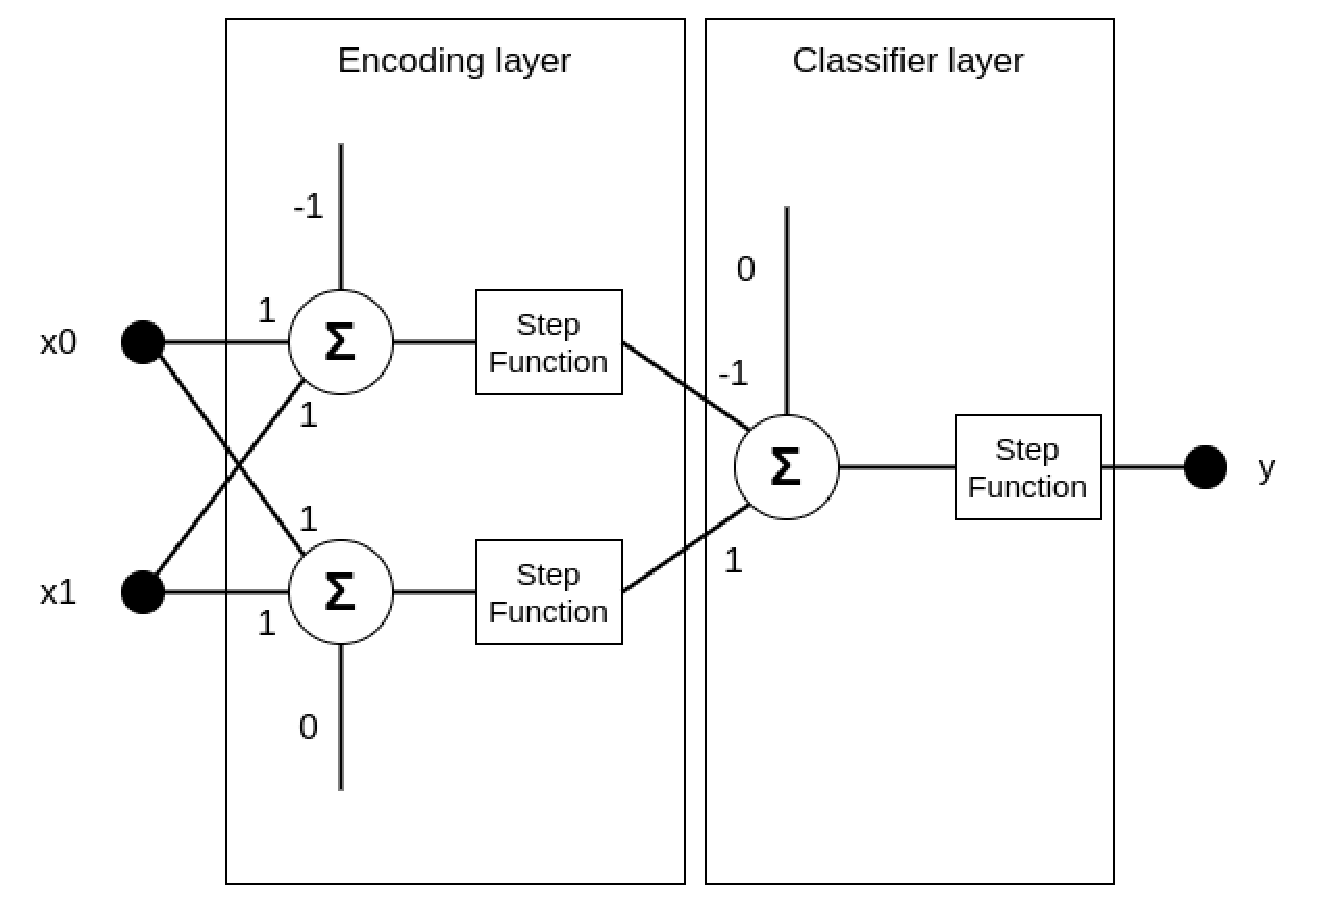
\includegraphics[width=\textwidth]{figures/neuro_xor}
	\caption{Neuron based equivalent of XOR function}
\end{figure}

%----------------------------------------------------------------------------------------------------
\subsection{Simple recurrent neural networks}
Simple solution to problem of time independence is to concatenate response of neural layer
from previous cycle to it input 
\begin{equation}
	\label{equ:sru_input}
	x'(t)=[x(t)|y(t-1)]
\end{equation}
Such solution results in signal propagating trough time and influencing responses of future cycles,
if this is only modification to feed forward model such layer is called simple recurrent
unit (SRU).
While this solution makes model time aware it have its own problems, mainly a signal vanishing
issue. Since the input signal from cycle $n$ have direct influence only on a response of this
cycle and for each subsequent cycles it is only trough feedback loop. Influence of input $n$ on
response of cycle $n+k$ grows inverse proportional to $k$.
This means that in this model only those regularities that appear over short time periods can
be detected.
Making weights on feedback bigger will not eliminate problem and instead replace it with signal
explosion that causes response to reach maximum value if a strong signal appeared on input at
least once.

%----------------------------------------------------------------------------------------------------
\subsection{Networks with long term memory}
One of possible solutions to this issue is addition of long term memory which will regulate
forward and loop back path influence on neuron response, such solution is used in long short
term memory (LSTM) networks \cite{Hochreiter1997}.
\begin{figure}[htb] 
	\label{fig:lstm}
	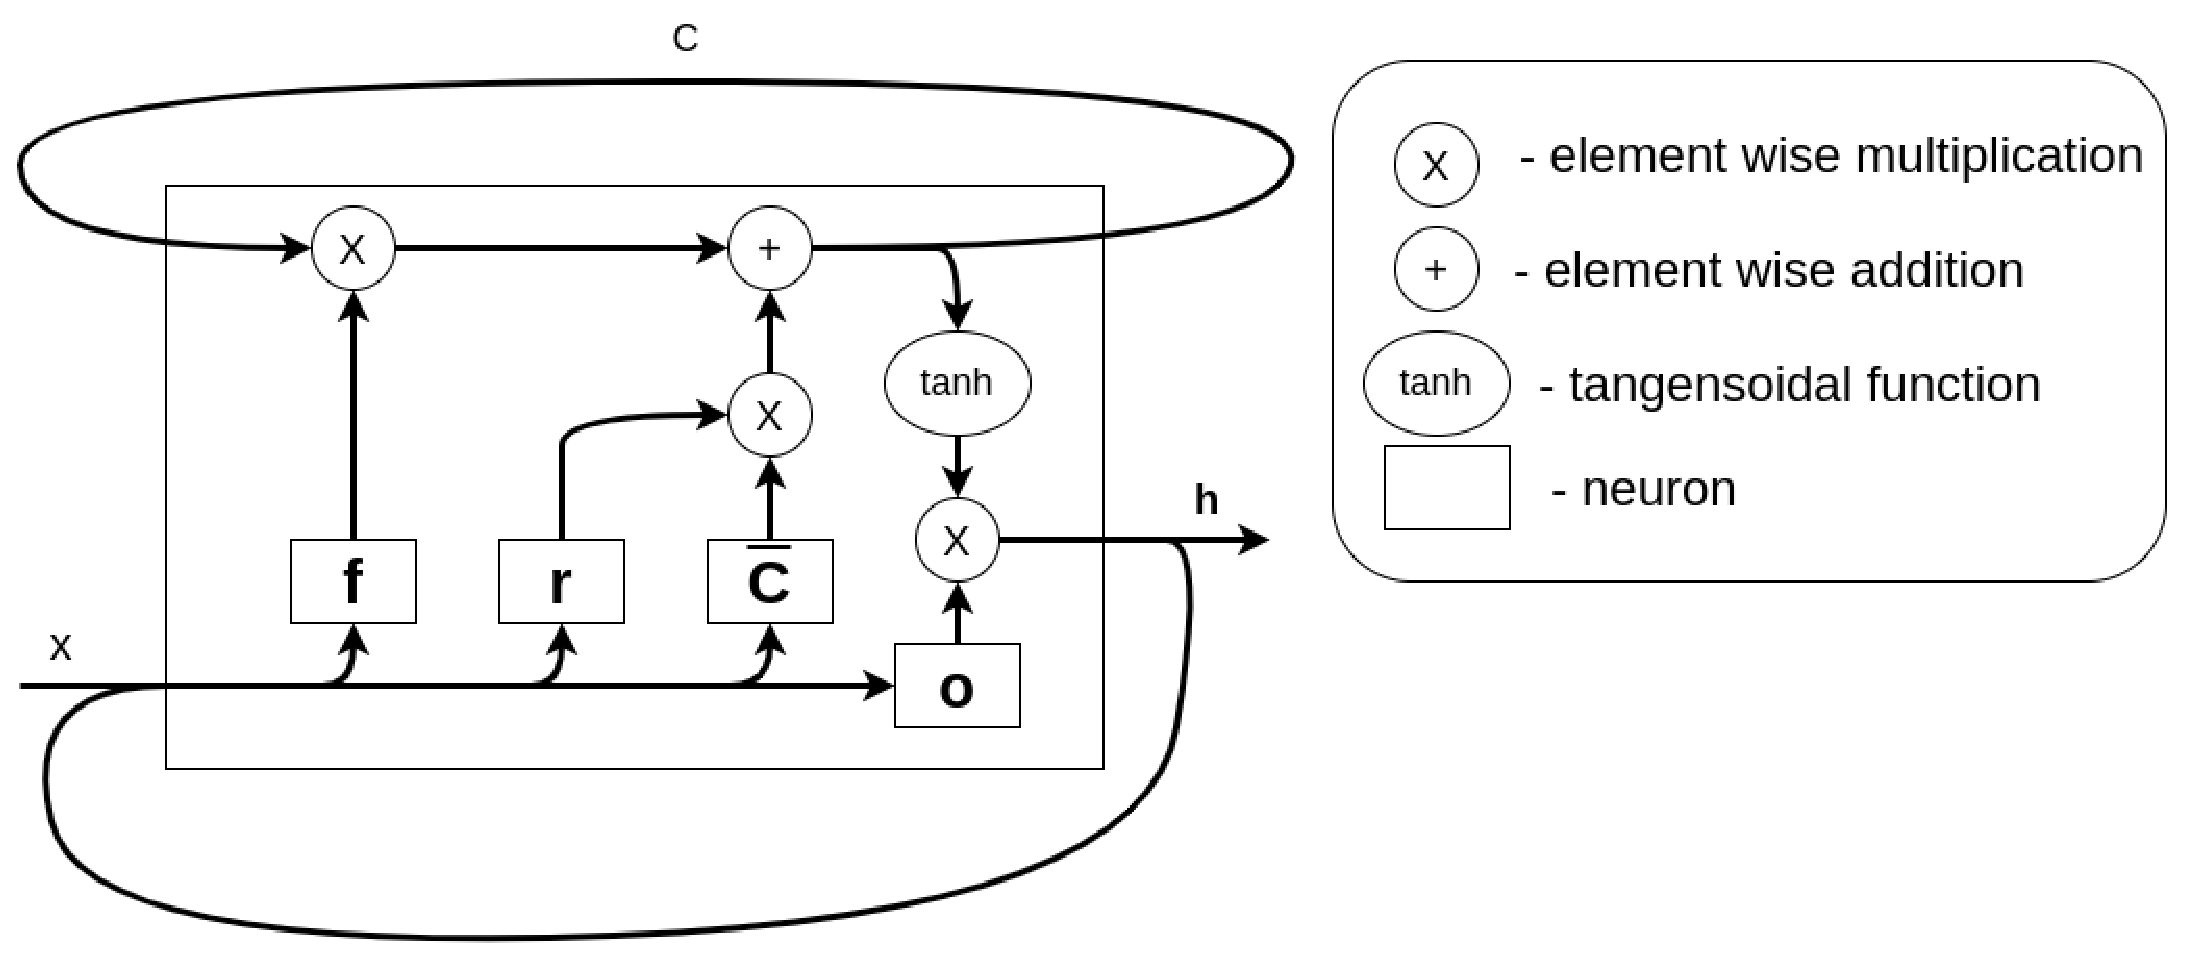
\includegraphics[width=\textwidth]{figures/lstm}
	\caption{LSTM layer}
\end{figure}
Single LSTM neuron consists of 4 basic neurons and two non neuron operations:
\begin{itemize}
\item $x'(t)=[x(t)|y(t-1)]$,
\item $o_t=\sigma (W_o\cdot x'_t+b_o)$,
\item $r_t=\sigma (W_r\cdot x'_t+b_r)$,
\item $f_t=\sigma (W_f\cdot x'_t+b_f)$,
\item $\bar{C}_t=\tanh (W_c\cdot x'_t+b_c)$,
\item $C_t=f_t\circ C_{t-1}+r_t\circ \bar{C}_t$,
\item $y_t=o_t\circ \tanh (C_t)$.
\end{itemize}
With $W$ and $b$ being weights and biases for each basic neuron, $x$ input, $y$ output and
$C$ long term memory. As it can be seen $o_t$ is a equivalent of SRU and is moderated by
long term memory before propagating as output. Temporary value of long term memory based
only on current output $\bar{C}_t$ is calculated and then with help of neurons $r$ and $f$
is transformed into its final value.
Neuron $r$ is called remembering gate and influences to what degree temporary long term
memory from given cycle effects its final value while $f$ is forgetting gate and
decides influence of long term memory from last cycle on current one.
Thanks to such implementation model can learn to detect long term regularities as well
as short term ones.

